\section{Determinación de la Demanda}%
\label{sec:Determinación de la Demanda}

A partir del conjunto de datos \cite{Nacional2016}, se obtuvo una lista de 2404
instituciones educativas públicas y privadas en Bogotá.
Dicha información contaba con características de interés que incluían el nombre
de la institución; la zona (rural, urbana o ambas);
el nivel (primaria, secundaria, preescolar, etc.); la especialidad
(académica, industrial, comercial); los grados (primero, segundo, octavo,
etc.); el idioma (adicionales al español); y el tipo de servicio (público,
privado o mixto).

Los datos se filtraron para considerar únicamente instituciones con educación
secundaria (nivel), que impartieran grados entre octavo y undécimo, con
especialidad académica y de tipo privado.
La justificación para la selección de estos grados radica en que los
estudiantes de mayor edad poseen la madurez y el bagaje de conocimientos
necesarios para trabajar eficazmente con los dispositivos.
Por su parte, la elección de instituciones privadas se debe a consideraciones
de financiamiento, como se estableció previamente.

Este proceso de selección redujo el número de instituciones de 2404 a 565
posibles.
Dado que esta cifra seguía siendo elevada, se aplicó un filtro adicional
utilizando el modelo de enseñanza, enfocándose exclusivamente en instituciones
no orientadas a nivelación o a la educación para adultos.
Asimismo, se descartaron las instituciones con calendario B, debido al desfase
temporal con los horarios de los integrantes del equipo del proyecto.
Con la información obtenida de la base de datos del Ministerio de Educación,
el número mínimo posible de instituciones identificadas fue de 490.

De esta lista de instituciones, se realizó un proceso de web scraping y se
consultaron sus respectivos sitios web.
Se seleccionaron aquellas que hacían mención explícita a ``STEM'', ``énfasis en
ciencias'' o ``astronomía'', resultando en una lista final de 238 instituciones.

Con base en estos resultados, estimamos una demanda potencial para nuestro
proyecto de aproximadamente 270 instituciones.
Esta estimación considera la posible existencia de datos faltantes durante los
procesos de filtrado y web scraping.
En una ciudad con más de 2400 instituciones educativas, esto representa
aproximadamente un 11\% del mercado potencial.

\begin{figure}
  \centering
  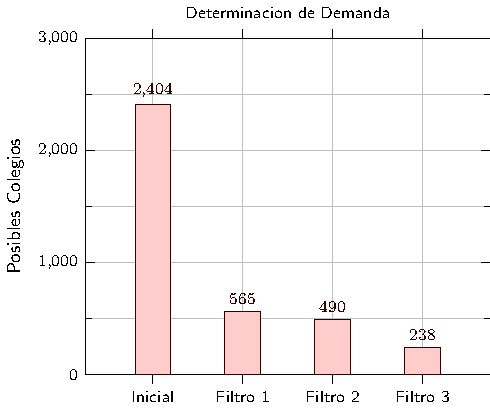
\includegraphics[width=0.75\linewidth]{./Figures/bar-plot-demand.pdf}
  \caption{Determinación de la demanda según filtro.}
\end{figure}

A partir de la base de datos, se observa que la cantidad de instituciones es
estable, no se generan nuevas instituciones ya que la cantidad de estudiantes
va rotando.
Por ello se toma que la demanda no cambiara en los próximos 5 años.
